\begin{figure}[t]
\vspace{-0.1in}
    \centering
    \raisebox{\baselineskip}%
    {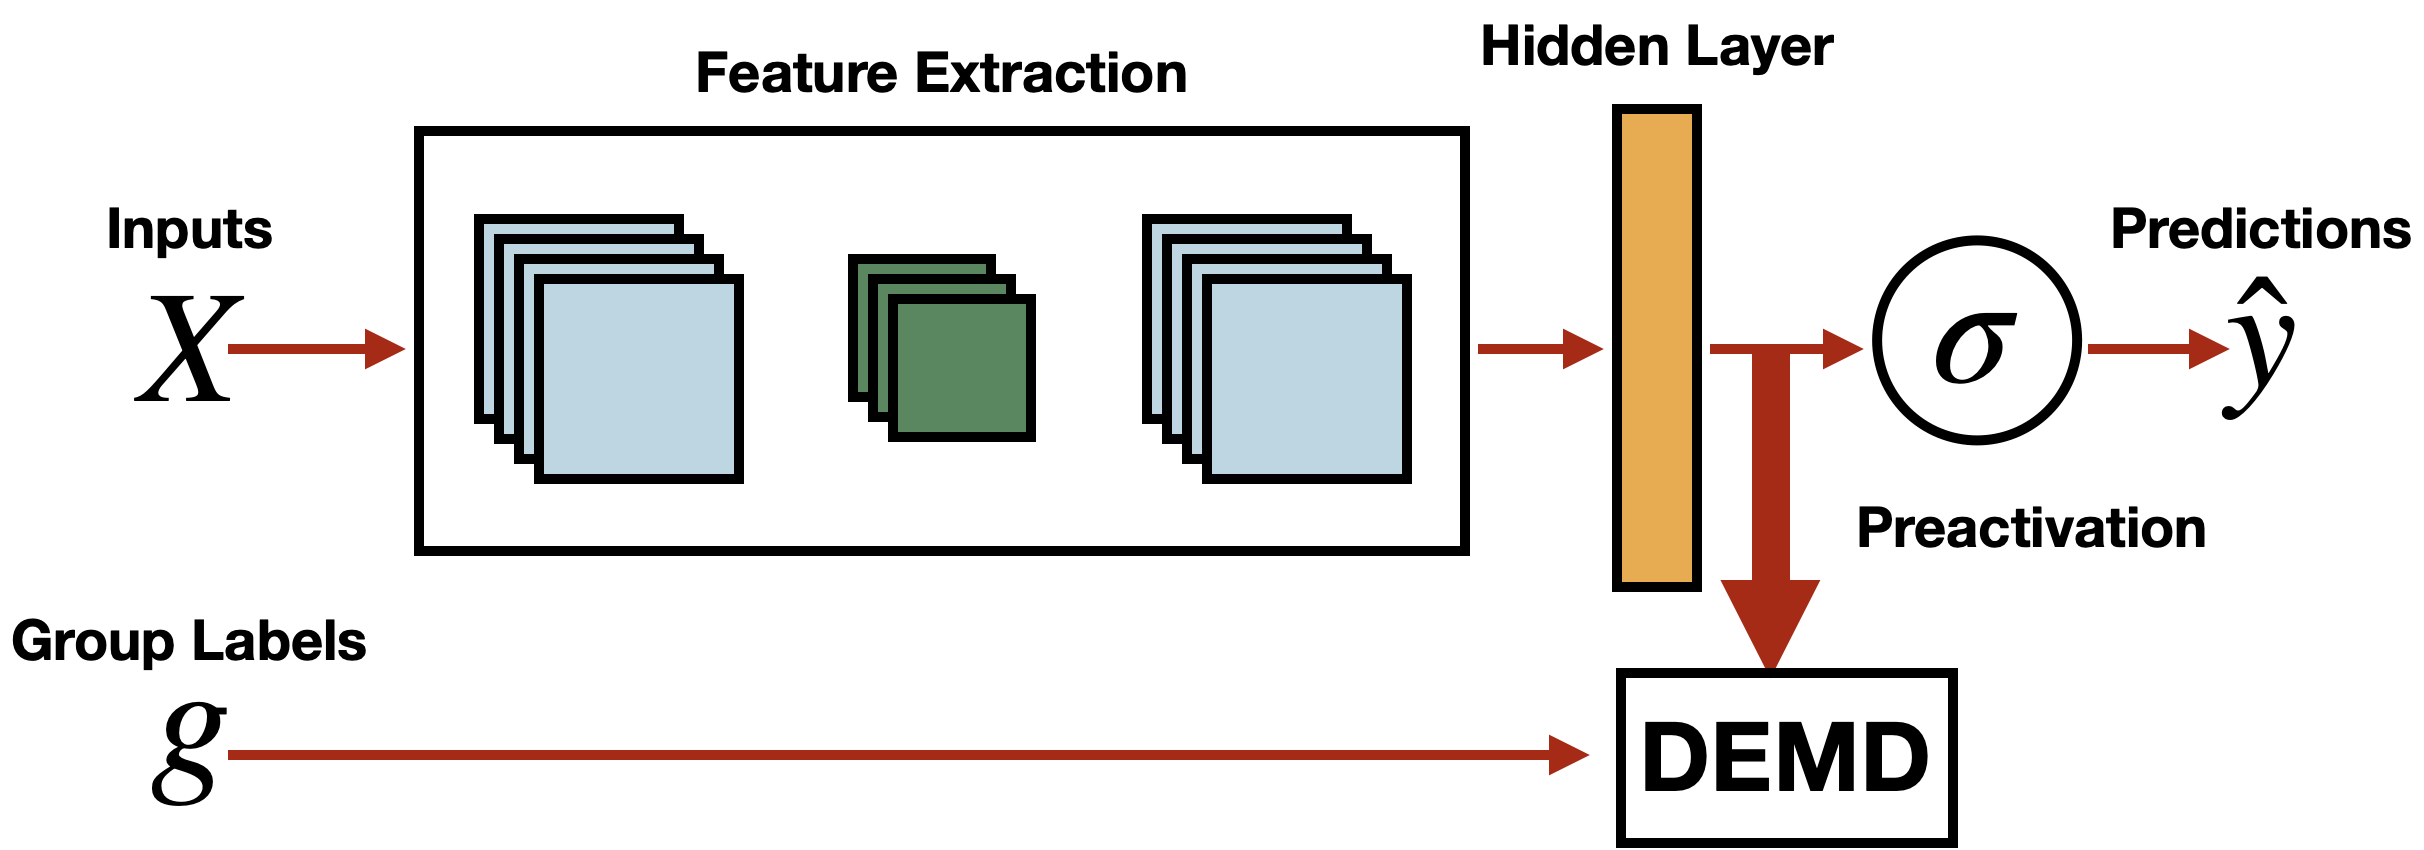
\includegraphics[width=0.55\columnwidth]{6_demd/figs/net_diff_new.png}%
    }% 
    \;
    \includegraphics[width=0.35\columnwidth]{6_demd/figs/Distance_Comparisons.pdf}
    \caption[DEMD regularization and computation speedups]{\label{fig:dists} (Left) DEMD is positioned after the final layer, prior to the activation. Activations are sorted into distributions utilizing group labels provided alongside the input data. Computed distributions are then brought together using our algorithm. (Right) Computation times for direct distance evaluation of EMD-like distances. Existing methods take much more time {\color{blue}(check $y$-axis)} as the number of distributions grow.}
    \vspace{-5pt}
\end{figure}

\section{Numerical Evaluations and Fairness Experments}
\label{sec:results}
\vspace{-5pt}
% \subsection{Implementation Details}
% While accounting for dual variables in practice is relatively easy, we may directly take advantage of existing automatically computed gradients from existing software to avoid the bookkeeping and tracking of dual variables entirely. While these gradients may not exactly equal the dual variables, they are directions of descent with respect to our distributions of interest, and are equally sufficient for our purposes.

% Traditional analysis and learning pipelines do not consist of binned distributions, but rather empirical distributions over real-numbered outputs. For this reason it is necessary that we construct a differentiable histogramming operation, that will allow gradients computed with respect to the dEMD measure to flow backwards on a per-sample or per-batch basis. 

% \vishnu{I feel these details are not necessary in the main paper. } Experiments were conducted using NumPy and PyTorch on a Intel(R) Xeon(R) CPU E5-2620 v3 @ 2.40GHz with an Nvidia Titan Xp GPU. 
We evaluate our construction in a number of settings. 
First, we demonstrate the computational speedup associated with evaluating d-MMOT using our algorithm, along with speedups associated with directly computing the gradient.
Next, we compute the construction in a series of neural network tasks associated with ensuring distributional similarity: fairness, invariant representations, and multi-domain matching.
We provide a complete PyTorch Network Module that packages the above differentiable DEMD objective and histogram functions,
and serves as a plug-and-play regularization module. %\vishnu{One major criticism in the experiments is we don't evaluate in a setting where there are too many distributions to match. }


\subsection{Performance Benchmarks}

Figure \ref{fig:speeds} presents NumPy and Torch instantiations of both forward and backward passes using automatic differentiation and the gradients computed using the dual as in Section \ref{sec:dual}. As expected, the forward (distance computation) times are comparable, but the backwards computation scales poorly with the number of distributions to be updated using automatic differentiation. Our dual setting allows the gradients to simply be read off (based on the forward pass), leading to \textbf{no} additional computation overhead during backpropagation.
\begin{figure}
    \centering
    \fbox{
    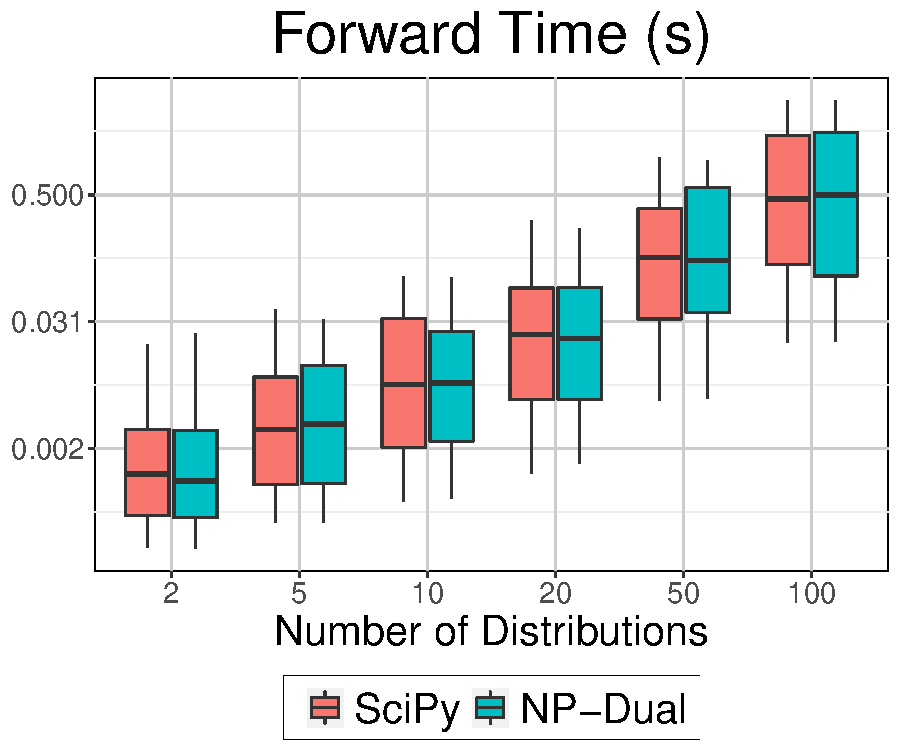
\includegraphics[width=0.22\textwidth]{6_demd/figs/fwbk_new/Numpy_Forwards_10Bins.pdf}
    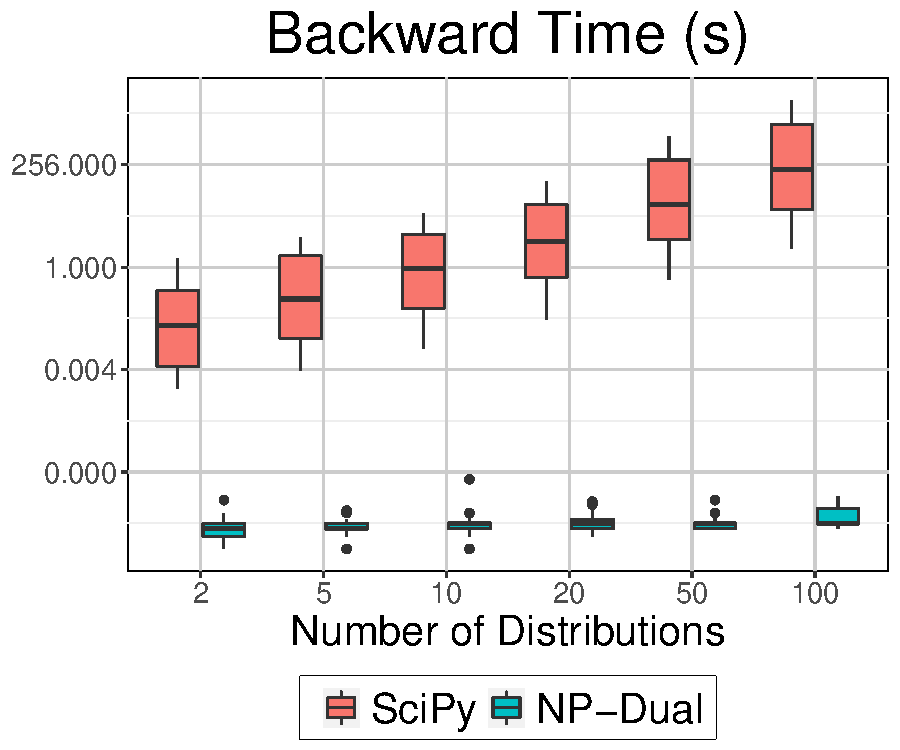
\includegraphics[width=0.22\textwidth]{6_demd/figs/fwbk_new/Numpy_Backward_10Bins.pdf}
    }%
    \;
    \fbox{
    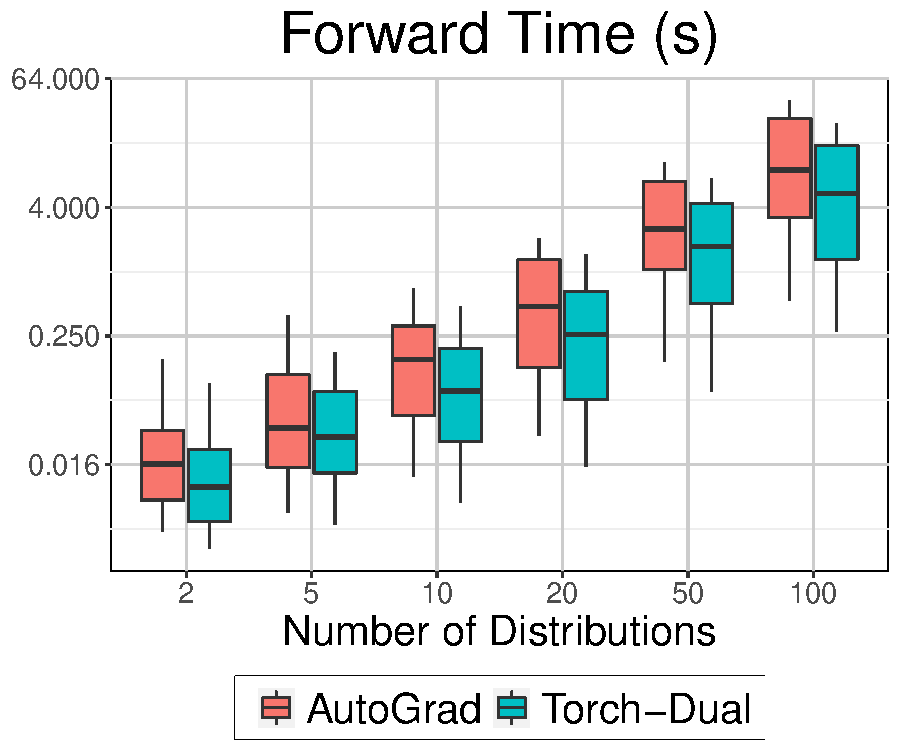
\includegraphics[width=0.22\textwidth]{6_demd/figs/fwbk_new/Torch_Forwards_10Bins.pdf}
    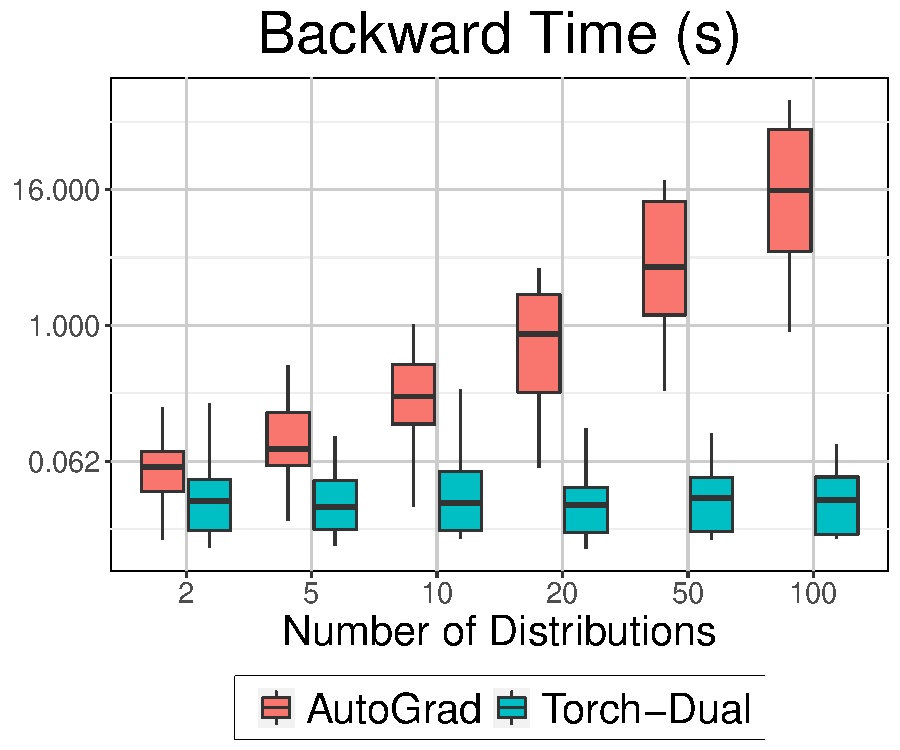
\includegraphics[width=0.22\textwidth]{6_demd/figs/fwbk_new/Torch_Backward_10Bins.pdf}
    }%
    \caption[DEMD forward and backward time copmarisons]{Forward/Backward Pass Times for 10 Bins with varying number of distributions, averaged over 10 runs. Forward wall-clock times are comparable, regardless of backend ({\em left pair}: NumPy+SciPy; {\em right pair}: PyTorch+AutoGrad). Direct reading of the gradient via the dual leads to significant gains in backward pass times, where automatic differentiation scales poorly with the number of distributions.}
    \label{fig:speeds}
\end{figure}


% \subsection{Comparing Methods for Optimal Transport with Monge Metrics}
We compare our DEMD computation 
%of the Earth Mover's Distance 
to what one may use given existing Optimal Transport methods in Figure \ref{fig:dists} (right). Using standard off-the-shelf methods as a baseline, when the cost is Monge our algorithm provides \textit{significant} speedups in computation time, on the scale of orders of magnitude! Further, if the number of distributions and bins increases, the time-cost for existing methods using more generic LP solvers can become significant, and may become infeasible with generic solutions via CVXPY \citep{diamond2016cvxpy}. 
% Figure \ref{fig:dists} shows the time dependence as the number of distributions grows, with 10 bins. 
We compare our approach to two off-the-shelf implementations of barycenters via the Python Optimal Transport (POT) Library \citep{flamary2021pot}, along with 
directly solving the Earth Mover's problem via CVXPY. 
Even for 10 distributions over 10 bins, CVXPY is unable to allocate the necessary memory using a direct instantiation.

% \begin{figure}
%     \centering
%     \includegraphics[width=0.45\columnwidth]{figs/Distance_Comparisons.pdf}
%     \caption{Times for direct distance computation of EMD-like distances. See text for details.}
%     \label{fig:dists}
% \end{figure}

%% Barycenters doesnt work right now
% \subsection{Common Barycenter Computations and Comparisons}
% -comparing with Cuturi and janati here, working on setup with janati code

% \begin{figure}
%     \centering
%     \includegraphics[width=0.8\columnwidth]{example-image-a}
%     \caption{Comparison of approaches against DEMD over ellipse barycenters.}
%     \label{fig:}
% \end{figure}


%\section{Traditional methods for optimizing fairness: How do we compare?}
% \subsection{Example Applications}
% Here we instantiate the full setting as described in Section \ref{sec:fair}, and compare to existing drop-in regularizers meant to account for fairness. Because our approach operates on the activations prior to classification, we first compare our method using only two bins defined as above or below 0.5, so as to directly mimic the classification metric used in existing setups.

% \subsection{MNIST}
% Using the MNIST handwritten digit dataset, we construct a new classification problem. The distribution of digit size within the frame is typically the same; we augment the dataset with ``small" and ``large" versions of the digits within a single frame, and define a classification problem over determining the size of the digit within the frame. An ideal size classifier in this case should be agnostic to the digit being classified as large or small.

% \begin{figure}
%     \centering
%     \includegraphics[width=0.8\columnwidth]{example-image-b}
%     \caption{Effect of varying DEMD regularization weight, accuracy across groups.}
%     \label{fig:mnist}
% \end{figure}

\subsection{Generalized EM Fairness on Fairness Datasets}
With a viable tool in hand, we move to practical applications in machine learning fairness,
which naturally requires
enforcing closeness in model outputs.
Here, we construct networks with our DEMD regularizer,
where we discretize the final activation output
prior to classification,
and push the distributions of this activation to be similar
among sensitive attributes.

\paragraph{Data.}
We identify 4 common fairness datasets often used to benchmark
fair machine learning algorithms: (1) the German Credit Dataset \citep{german}, (2) the Adult Income Dataset \citep{uci}, (3) the Communities and Crime Dataset \citep{crime}, and (4) The ACS Income dataset, recently made available as a large, population-level demographic dataset \citep{ding2021retiring} containing as many as nine sensitive attributes. We set up a simple three-layer neural network for classification tasks with the addition of a fairness-type regularizer. We compare our construction with 4 off-the-shelf plug-in regularizers: (1) No regularization, (2) Demographic Parity (DP), (3) Equalized Odds (EO), and (4) a histogrammed barycenter construction. DP and EO regularizers were computed using a PyTorch version of FairLearn \citep{bird2020fairlearn}, and the barycenter version was implemented using POT library (with GPU backend). Because the scale of the regularization term is not directly comparable, we sweep regularization weights and select the best over all measures for a each dataset/regularizer pair. 
We use 10 bins and replicate all experiments over three random seeds.

% The American Census Survey (ACS) has recently made available a large set of demographic data. The original UCI Adult dataset \cite{uci} was curated from this data, however recent work by \cite{ding2021retiring} has identified temporal shifts in demographic data, and recommends using a more recent collection as a baseline when evaluating biases and adjusting for fairness. Part of their contribution includes APIs to directly interface with the data provided by the ACS, and the ability to identify and construct similar problems associated with the original UCI-provided dataset, albeit with updated data. Data for the income prediction task was downloaded from 2018, localized to California. After preprocessing, 195665 samples were split: 75\% training and 25\% validation. Race is the provided group label, which we wish to be agnostic toward over some measure of our output.
\paragraph{Models.} We set up two model settings with a standard logistic regressor and a 2-layer neural network. We compare three types of plug-in regularizers: (1) Demographic Parity (DP), (2) Equalized Odds (EO), and (3) the Generalized EMD. DP and EO regularizers were computed using a PyTorch implementation of FairLearn \citep{bird2020fairlearn}. 
%Since the scale of the regularization term in our measure is not directly comparable, we sweep over the regularization weights. 

\paragraph{Results.} In the summary in Table~\ref{tab:fair_results}, models were selected with the largest regularization weight before accuracy dropped significantly. When accuracies are comparable, we see good performance (when minimizing DEMD regularizer) against baseline methods. Notably, when accuracies are similar across methods, minimizing DEMD tends to give better (lower) fairness measures across all datasets.
{\bf Summary:} DEMD on the final network layer helps control multiple fairness measures.


% First we see that sweeps over regularization weights act as expected for our metric, as well as for existing fairness measures. 
% Table~\ref{tab:acsinc2} show results after training with a large range of regularization weights.
% Training models with no regularization leads to significantly different accuracies over race groups within the data, and strong regularization reduces both the EMD distance and traditional fairness measures over the output via demographic parity (DP) and equality of opportunity (EO). Table~\ref{fig:reg_sweep} shows a particular tighter sweep for EMD regularizer with 10 bins used as the discretization level, closer to the region with large swings in the trade-off. Close correspondence with DP and EO measured after thresholding suggests the model may be robust to choices in the selection threshold.
% Validation results for various models and regularization weights on the ACS Income prediction task including demographic parity
% (DP) and equality of opportunity (EO) spreads. In this setting only two bins are used for direct comparison to output-style regularizers.


\begin{table*}[!t] 
	\scriptsize
	\setlength\tabcolsep{3.5pt} % make LaTeX figure out width of inter-column spaces
	\caption[Fairness application comparisons using DEMD regularization]{\textbf{Fairness Experiments.} Measures evaluated using standard metrics: maximum Demographic Parity Gap \textbf{(DP)},  maximum Equalized Odds Gap \textbf{(EO)}, and \textbf{(DEMD)}. For all measures, lower values are preferred.  With comparable accuracy, DEMD regularization leads to fairer representations as measured by common metrics. DP and EO measures are scaled by 100 for ease of presentation. Best results shown in bold.}
	\begin{tabular*}{\linewidth}{l *{3}{c}|*{3}{c}|*{3}{c}|*{3}{c}}
		\midrule%\midrule
		& \multicolumn{3}{c}{German} & \multicolumn{3}{c}{Adult} & \multicolumn{3}{c}{Crime}& \multicolumn{3}{c}{ACS-Income} \\
		\cmidrule{2-4} \cmidrule{5-7} \cmidrule{8-10} \cmidrule{11-13}
		& DP & EO & DEMD & DP & EO & DEMD & DP & EO & DEMD & DP & EO & DEMD \\ 
		\midrule
% 		None & 0.180 & 0.134 & 1.694 & 0.382 & 0.446 & 2.858 & 0.351 & 0.306 & 3.556 & 0.365 & 0.251 & 4.778 \\
% DP-Reg. & 0.169 & 0.128 & 1.600 & 0.383 & 0.446 & 2.832 & 0.362 & 0.250 & 3.705 & 0.477 & 0.276 & 5.024 \\
% EO-Reg. & 0.143 & 0.116 & 1.425 & 0.377 & 0.442 & 2.830 & 0.363 & 0.311 & 3.055 & 0.377 & 0.256 & 4.818 \\
% Bary & 0.177 & 0.134 & 1.645 & 0.362 & 0.442 & 2.811 & 0.377 & 0.256 & 2.726 & 0.571 & 0.497 & 4.376 \\
% DEMD & 0.145 & 0.117 & 1.443 & 0.364 & 0.438 & 2.688 & 0.288 & 0.361 & 3.101 & 0.334 & 0.236 & 3.598 \\
None & $17\scriptscriptstyle(5)$ & $11\scriptscriptstyle(2)$ & $1.69\scriptscriptstyle(0.32)$ & $18\scriptscriptstyle(1)$ & $13\scriptscriptstyle(0)$ & $1.69\scriptscriptstyle(0.07)$ & $38\scriptscriptstyle(6)$ & $45\scriptscriptstyle(3)$ & $2.86\scriptscriptstyle(0.38)$ & $37\scriptscriptstyle(1)$ & $25\scriptscriptstyle(0)$ & $4.78\scriptscriptstyle(0.32)$ \\
DP-Reg. & $16\scriptscriptstyle(6)$ & $10\scriptscriptstyle(3)$ & $1.5\scriptscriptstyle(0.26)$ & $17\scriptscriptstyle(1)$ & $13\scriptscriptstyle(1)$ & $1.6\scriptscriptstyle(0.07)$ & $38\scriptscriptstyle(6)$ & $45\scriptscriptstyle(3)$ & $2.83\scriptscriptstyle(0.39)$ & $48\scriptscriptstyle(4)$ & $28\scriptscriptstyle(0)$ & $5.02\scriptscriptstyle(0.31)$ \\
EO-Reg. & $17\scriptscriptstyle(5)$ & $11\scriptscriptstyle(2)$ & $1.69\scriptscriptstyle(0.32)$ & $\textbf{14}\scriptscriptstyle(1)$ & $\textbf{12}\scriptscriptstyle(1)$ & $\textbf{1.43}\scriptscriptstyle(0.07)$ & $38\scriptscriptstyle(5)$ & $\textbf{44}\scriptscriptstyle(3)$ & $2.83\scriptscriptstyle(0.39)$ & $38\scriptscriptstyle(1)$ & $26\scriptscriptstyle(0)$ & $4.82\scriptscriptstyle(0.32)$ \\
Bary-POT & $27\scriptscriptstyle(5)$ & $17\scriptscriptstyle(1)$ & $1.5\scriptscriptstyle(0.21)$ & $18\scriptscriptstyle(1)$ & $13\scriptscriptstyle(0)$ & $1.64\scriptscriptstyle(0.07)$ & $\textbf{36}\scriptscriptstyle(5)$ & $\textbf{44}\scriptscriptstyle(4)$ & $2.81\scriptscriptstyle(0.3)$ & $57\scriptscriptstyle(37)$ & $50\scriptscriptstyle(44)$ & $4.38\scriptscriptstyle(0.16)$ \\
DEMD (ours) & $\textbf{14}\scriptscriptstyle(7)$ & $\textbf{9}\scriptscriptstyle(4)$ & $\textbf{1.41}\scriptscriptstyle(0.35)$ & $15\scriptscriptstyle(1)$ & $\textbf{12}\scriptscriptstyle(1)$ & $1.44\scriptscriptstyle(0.08)$ & $\textbf{36}\scriptscriptstyle(6)$ & $\textbf{44}\scriptscriptstyle(3)$ & $\textbf{2.69}\scriptscriptstyle(0.44)$ & $\textbf{33}\scriptscriptstyle(0)$ & $\textbf{24}\scriptscriptstyle(0)$ & $\textbf{3.6}\scriptscriptstyle(0.29)$ \\
		\midrule%\midrule
	\end{tabular*}
	\label{tab:fair_results}
\end{table*} 

\subsection{Harmonization for Invariant Representations}
Having evaluated the use of the DEMD layer to constrain the neural network for  fairness measures, we will now move to a more general problem of deriving invariant representations from the datasets. Here, invariance is sought in regard to the sensitive attributes. Recent works \citep{equivar} on invariant representation learning propose leveraging an encoder-decoder architectures to map the dataset features to latent space representations. The latent space representations are penalized to match or harmonize the distributions across several groups in the dataset. In contrast to the previous section, the goal here is to identify a good mapping in the latent space that is devoid of any group-related information in the dataset.  Consequently, our evaluation metrics test if the latent representations have a lower value of (i) ADV, adversarial measure and (ii) MMD, maximum mean discrepancy measure. The measure ADV tests to what extent can a separate neural network predict the group information from the latent features. Alternatively, the MMD scores measure the distance between the probability distributions across groups. Prior works such as \cite{zemel} and \cite{cai} optimize each of these measures separately. Our experiments (Table~\ref{tab:harm_results}) show the DEMD layer performs competitively with the baselines when applied on the latent space. Interestingly, these performance gains come despite not directly optimizing the harmonization measures, in contrast to baselines, which require several practical adjustments (batch variants and secondary neural networks).
\textbf{Summary}: DEMD as an intermediate layer can be used to derive invariant representations efficiently.
% \vishnu{Need to convey a message that the baseline directly optimizes for the ADV and MMD measures. Our although doesn't directly optimizes these measures, still achieves competitive values on them. }
%Due to skewness amongst the groups, ROC-AUC is used to report the ADV measure on German dataset.
\begin{table*}[!t] 
	\scriptsize
	\setlength\tabcolsep{2.25pt} % make LaTeX figure out width of inter-column spaces
	\caption[Harmonization application comparisons using DEMD regularization]{\textbf{Harmonization Experiments.} Evaluations conducted along three metrics, Accuracy \textbf{(ACC)}, Adversarial measure \textbf{(ADV)} and Maximum Mean Discrepancy \textbf{(MMD)}. A lower value $\downarrow$ of ADV and MMD indicate successful harmonization across the different groups. A higher ACC with a small drop from baseline is preferred. }
	\begin{tabular*}{\linewidth}{l *{3}{c}|*{3}{c}|*{3}{c}|*{3}{c}}
		\midrule%\midrule
		& \multicolumn{3}{c}{German} & \multicolumn{3}{c}{Adult} & \multicolumn{3}{c}{Crime}& \multicolumn{3}{c}{ACS-Income} \\
		\cmidrule{2-4} \cmidrule{5-7} \cmidrule{8-10} \cmidrule{11-13}
		& ACC $\uparrow$ & ADV $\downarrow$ & MMD $\downarrow$ & ACC $\uparrow$ & ADV $\downarrow$ & MMD $\downarrow$ & ACC $\uparrow$ & ADV $\downarrow$ & MMD $\downarrow$ & ACC $\uparrow$ & ADV $\downarrow$  & MMD $\downarrow$ \\ 
		\midrule
		None & $74\scriptscriptstyle(0.9)$ & $93\scriptscriptstyle(1.3)$ & $7.7\scriptscriptstyle(0.8)$ & $84\scriptscriptstyle(0.1)$ & $83\scriptscriptstyle(0.1)$ & $9.8\scriptscriptstyle(0.3)$ & $85\scriptscriptstyle(0.2)$ & $77\scriptscriptstyle(0.5)$ & $14\scriptscriptstyle(0.1)$ & $78\scriptscriptstyle(0.1)$ & $98\scriptscriptstyle(0.7)$ & $160\scriptscriptstyle(2)$ \\
		Li et al. & $73\scriptscriptstyle(1.5)$ & $92\scriptscriptstyle(1.3)$ & $1.5\scriptscriptstyle(0.3)$ & $84\scriptscriptstyle(0.1)$ & $83\scriptscriptstyle(0.1)$ & $3.1\scriptscriptstyle(0.3)$ & $85\scriptscriptstyle(0.5)$ & $76\scriptscriptstyle(1.6)$ & $12\scriptscriptstyle(1.0)$ & $78\scriptscriptstyle(0.1)$ & $97\scriptscriptstyle(0.5)$ & $17\scriptscriptstyle(1.2)$ \\
		Xie et al. & $76\scriptscriptstyle(1.3)$ & $93\scriptscriptstyle(0.6)$ & $1.2\scriptscriptstyle(0.2)$ & $84\scriptscriptstyle(0.04)$ & $81\scriptscriptstyle(0.7)$ & $4.2\scriptscriptstyle(2.4)$ & $85\scriptscriptstyle(0.2)$ & $76\scriptscriptstyle(0.7)$ & $15\scriptscriptstyle(0.6)$ & $78\scriptscriptstyle(0.1)$ & $94\scriptscriptstyle(5.6)$ & $99\scriptscriptstyle(2.9)$ \\
		DEMD & $74\scriptscriptstyle(1.1)$ & $93\scriptscriptstyle(0.4)$ & $2.1\scriptscriptstyle(0.4)$ & $84\scriptscriptstyle(0.03)$ & $82\scriptscriptstyle(0.2)$ & $5.3\scriptscriptstyle(1.4)$ & $83\scriptscriptstyle(0.3)$ & $72\scriptscriptstyle(1.0)$ & $7.1\scriptscriptstyle(1.0)$ & $77\scriptscriptstyle(0.4)$ & $96\scriptscriptstyle(0.5)$ & $26\scriptscriptstyle(3.9)$ \\
		\midrule
	\end{tabular*}
	\label{tab:harm_results}
	%\vspace{-5pt}
\end{table*} 

% \scriptscriptstyle(XXX)
%%%% This is a copy of the table from vishnu, needs to be formatted properly
% \begin{table*}[!t] 
% 	\footnotesize
% 	\captionsetup{justification=centering} 
% 	\setlength\tabcolsep{0pt} % make LaTeX figure out width of inter-column spaces
% 	\caption*{$\boldsymbol{{\Delta}_{Eq}}:$  Equivariance Gap, $\boldsymbol{Adv}:$ Adversarial Test Accuracy, $\boldsymbol{\mathcal{M}}:$ Test  $\mathcal{MMD}$ measure, $\boldsymbol{\mathcal{ACC}}:$ Test prediction accuracy\\
% 		$\uparrow$: Higher Value is preferred, $\downarrow$: Lower Value is preferred}
% 	\vspace{-4mm}
% 	\begin{tabular*}{\linewidth}{l @{\extracolsep{\fill}}
% 			*{24}{S[table-format=3.0]}}
% 		\midrule\midrule
% 		& \multicolumn{4}{c}{German} & \multicolumn{4}{c}{Adult} & \multicolumn{4}{c}{ADNI}& \multicolumn{4}{c}{ADCP} \\
% 		\cmidrule{2-5} \cmidrule{6-9} \cmidrule{10-13} \cmidrule{14-17}
% 		& {${\Delta}_{Eq}$ $\uparrow$} & {$Adv$ $\downarrow$} & {$\newsym{M}$ $\downarrow$} & \cellcolor{gray!25}{$\mathcal{ACC}$ $\uparrow$} & {${\Delta}_{Eq}$ $\uparrow$} & {$Adv$ $\downarrow$} & {$\newsym{M}$ $\downarrow$} & \cellcolor{gray!25}{$\mathcal{ACC}$ $\uparrow$} & {${\Delta}_{Eq}$ $\uparrow$} & {$Adv$ $\downarrow$} & {$\newsym{M}$ $\downarrow$} & \cellcolor{gray!25}{$\mathcal{ACC}$ $\uparrow$} & {${\Delta}_{Eq}$ $\uparrow$} & {$Adv$ $\downarrow$} & {$\newsym{M}$ $\downarrow$} & \cellcolor{gray!25}{$\mathcal{ACC}$ $\uparrow$}  \\ 
% 		\midrule\midrule
% 		Na\"ive & {$4.6{\scriptscriptstyle(0.7)}$ } &  {$0.62{\scriptscriptstyle(0.03)}$ }  &  {$7.7{\scriptscriptstyle(0.8)}$}  &  \cellcolor{gray!25}{$74{\scriptscriptstyle(0.9)}$}  &  {$3.4{\scriptscriptstyle(0.7)}$}  &  {$83{\scriptscriptstyle(0.1)}$}  &  {$9.8{\scriptscriptstyle(0.3)}$}  &  \cellcolor{gray!25}{$84{\scriptscriptstyle(0.1)}$}  &  {$3.1{\scriptscriptstyle(1.0)}$}  &  {$59{\scriptscriptstyle(2.9)}$}  &  {$27{\scriptscriptstyle(1.6)}$}  &  \cellcolor{gray!25}{$80{\scriptscriptstyle(2.6)}$} &  {$4.1{\scriptscriptstyle(0.9)}$} &  {$49{\scriptscriptstyle(8.4)}$} &  {$90{\scriptscriptstyle(8.7)}$} &  \cellcolor{gray!25}{$83{\scriptscriptstyle(4.4)}$}    \\
% 		MMD \cite{li2014learning}  & {$4.5{\scriptscriptstyle(1.0)}$ }&  {$0.66{\scriptscriptstyle(0.04)}$}  &  {$1.5{\scriptscriptstyle(0.3)}$}  &  \cellcolor{gray!25}{$73{\scriptscriptstyle(1.5)}$}  &  {$3.4{\scriptscriptstyle(0.9)}$}  &  {$83{\scriptscriptstyle(0.1)}$}  &  {$3.1{\scriptscriptstyle(0.3)}$}  &  \cellcolor{gray!25}{$84{\scriptscriptstyle(0.1)}$} &  {$3.1{\scriptscriptstyle(1.0)}$}  &  {$59{\scriptscriptstyle(3.3)}$}  &  {$27{\scriptscriptstyle(1.7)}$}  &  \cellcolor{gray!25}{$80{\scriptscriptstyle(2.6)}$}   &  {$3.6{\scriptscriptstyle(1.0)}$} &  {$49{\scriptscriptstyle(11.9)}$} &  {$86{\scriptscriptstyle(11.0)}$} &  \cellcolor{gray!25}{$84{\scriptscriptstyle(6.5)}$}  \\ 
% 		CAI \cite{NIPS2017_8cb22bdd} & {$1.9{\scriptscriptstyle(0.6)}$ }&  {$0.65{\scriptscriptstyle(0.01)}$}  &  {$1.2{\scriptscriptstyle(0.2)}$}  &  \cellcolor{gray!25}{$76{\scriptscriptstyle(1.3)}$}  &  {$0.1{\scriptscriptstyle(0.0)}$}  &  {$81{\scriptscriptstyle(0.7)}$}  &  {$4.2{\scriptscriptstyle(2.4)}$}  &  \cellcolor{gray!25}{$84{\scriptscriptstyle(0.04)}$}  &  {$2.4{\scriptscriptstyle(0.7)}$}  &  {$61{\scriptscriptstyle(2.1)}$}  &  {$27{\scriptscriptstyle(1.5)}$}  &  \cellcolor{gray!25}{$74{\scriptscriptstyle(3.6)}$}   &  {$2.8{\scriptscriptstyle(1.6)}$} &  {$56{\scriptscriptstyle(6.9)}$} &  {$85{\scriptscriptstyle(12.3)}$} &  \cellcolor{gray!25}{$82{\scriptscriptstyle(5.1)}$} \\ 
% 		SS \cite{zhou2018statistical} & {$3.8{\scriptscriptstyle(0.5)}$ }&  {$0.70{\scriptscriptstyle(0.07)}$}  &  {$1.5{\scriptscriptstyle(0.6)}$}  &  \cellcolor{gray!25}{$76{\scriptscriptstyle(0.9)}$}  &  {$2.8{\scriptscriptstyle(0.5)}$}  &  {$83{\scriptscriptstyle(0.2)}$}  &  {$1.5{\scriptscriptstyle(0.2)}$}  &  \cellcolor{gray!25}{$84{\scriptscriptstyle(0.1)}$}  &  {$3.7{\scriptscriptstyle(0.5)}$}  &  {$57{\scriptscriptstyle(2.1)}$}  &  {$26{\scriptscriptstyle(1.6)}$}  &  \cellcolor{gray!25}{$81{\scriptscriptstyle(3.7)}$}   &  {$3.4{\scriptscriptstyle(1.3)}$} &  {$51{\scriptscriptstyle(6.7)}$} &  {$88{\scriptscriptstyle(14.6)}$} &  \cellcolor{gray!25}{$82{\scriptscriptstyle(3.5)}$} \\ 	
% 		RM \cite{motiian2017unified} & {$3.4{\scriptscriptstyle(0.4)}$ }&  {$0.66{\scriptscriptstyle(0.04)}$}  &  {$7.5{\scriptscriptstyle(0.9)}$}  &  \cellcolor{gray!25}{$74{\scriptscriptstyle(2.1)}$}  &  {$0.8{\scriptscriptstyle(0.1)}$}  &  {$82{\scriptscriptstyle(0.4)}$}  &  {$4.8{\scriptscriptstyle(0.7)}$}  &  \cellcolor{gray!25}{$84{\scriptscriptstyle(0.3)}$}  &  {$0.8{\scriptscriptstyle(0.9)}$}  &  {$52{\scriptscriptstyle(5.4)}$}  &  {$22{\scriptscriptstyle(0.6)}$}  &  \cellcolor{gray!25}{$78{\scriptscriptstyle(3.8)}$}   &  {$0.4{\scriptscriptstyle(0.5)}$} &  {$40{\scriptscriptstyle(4.7)}$} &  {$77{\scriptscriptstyle(13.8)}$} &  \cellcolor{gray!25}{$84{\scriptscriptstyle(5.3)}$} \\ 	
% 		Ours & {$\boldsymbol{6.4{\scriptscriptstyle(0.6)}}$ } &  {$\boldsymbol{0.54{\scriptscriptstyle(0.01)}}$}  &  {$2.7{\scriptscriptstyle(0.6)}$}  &  \cellcolor{gray!25}{$75{\scriptscriptstyle(3.3)}$}  &  {$\boldsymbol{5.3{\scriptscriptstyle(0.9)}}$}  &  {$\boldsymbol{75{\scriptscriptstyle(1.4)}}$}  &  {$7.1{\scriptscriptstyle(0.6)}$}  &  \cellcolor{gray!25}{$83{\scriptscriptstyle(0.1)}$} &  {$\boldsymbol{5.1{\scriptscriptstyle(1.2)}}$}  &  {$\boldsymbol{50{\scriptscriptstyle(4.2)}}$}  &  {$\boldsymbol{16{\scriptscriptstyle(7.2)}}$}  &  \cellcolor{gray!25}{$77{\scriptscriptstyle(4.8)}$} &  {$\boldsymbol{7.5{\scriptscriptstyle(1.2)}}$} &  {$49{\scriptscriptstyle(7.3)}$} &  {$\boldsymbol{70{\scriptscriptstyle(22.3)}}$} &  \cellcolor{gray!25}{$81{\scriptscriptstyle(1.8)}$}  \\ 
% 		\midrule\midrule
% 	\end{tabular*} 
% 	\captionsetup{justification=justified} 
% 	\caption{ \footnotesize  \textbf{Quantitative Results.} We show Mean(Std) results over multiple run. For our baselines, we consider a \textbf{Na\"ive} encoder-decoder model, learning  representations via minimizing the \textbf{MMD} criterion \cite{li2014learning} and Adversarial training \cite{NIPS2017_8cb22bdd}, termed as \textbf{CAI}. We also compare against Sub-sampling (\textbf{SS}) \cite{zhou2018statistical} that minimizes the MMD criterion separately for every age group, and  the RandMatch (\textbf{RM}) \cite{motiian2017unified} baseline that generates matching input pairs based on the Age and target label values. The SS and RM baselines discard subset of samples if a match across sites is not available. The measure $Adv$ represents the adversarial test accuracy except for the German dataset where ROC-AUC is used due to high degree of skew in the data.  } 
% 	\label{tab:results}
% 	\vspace{-0.3in}
% \end{table*} 
\subsection{Multi-domain Image Translation}
%\glenn{Its not totally clear how we are suing DEMD here. Is it that we are regularizing the feature distribution in a new domain to be close to a new domain, right?, we need to clarify this with a sentence or two}  
We apply our construction to a recent multi-marginal GAN framing of multi-domain image translation.
With the goal of learning a mapping for a source image to multiple target domains, a focal point of recent literature has been to reduce the computational requirements of training individual models for each target, and learn a concurrent matching problem over a number of shared parameters or networks. MWGAN \citep{cao2019multi} set up a Multiple Marginal Matching problem in this context.
Extending upon their key observation that inter-domain constraints can be measured via the gradients for each domain,
we instantiate our DEMD layer over the gradient norms computed for each sample in a batch per group.
Specifically, DEMD minimizes the differences between the distributions over the gradient norms across all target domains.
% \jeff{at this spot it works to put a word on why DEMD going to be useful.  also emphasize that DEMD is used as a drop-in replacement module}
% Results are in agreement with results using MWGAN.
Using a weight of 100 for both regularizers,
we observe similar performance when compared 
to the original MWGAN construction.
In Figure~\ref{fig:mwgan} we show a few samples generated over an image translation task on the CelebA dataset.
Here, we aim to translate original dataset images to ones with specific target attributes.
\textbf{Summary:} Multi-domain image translation can be conducted by adding a DEMD layer in the native GAN construction. 

% \begin{figure}
%     \centering
%     % 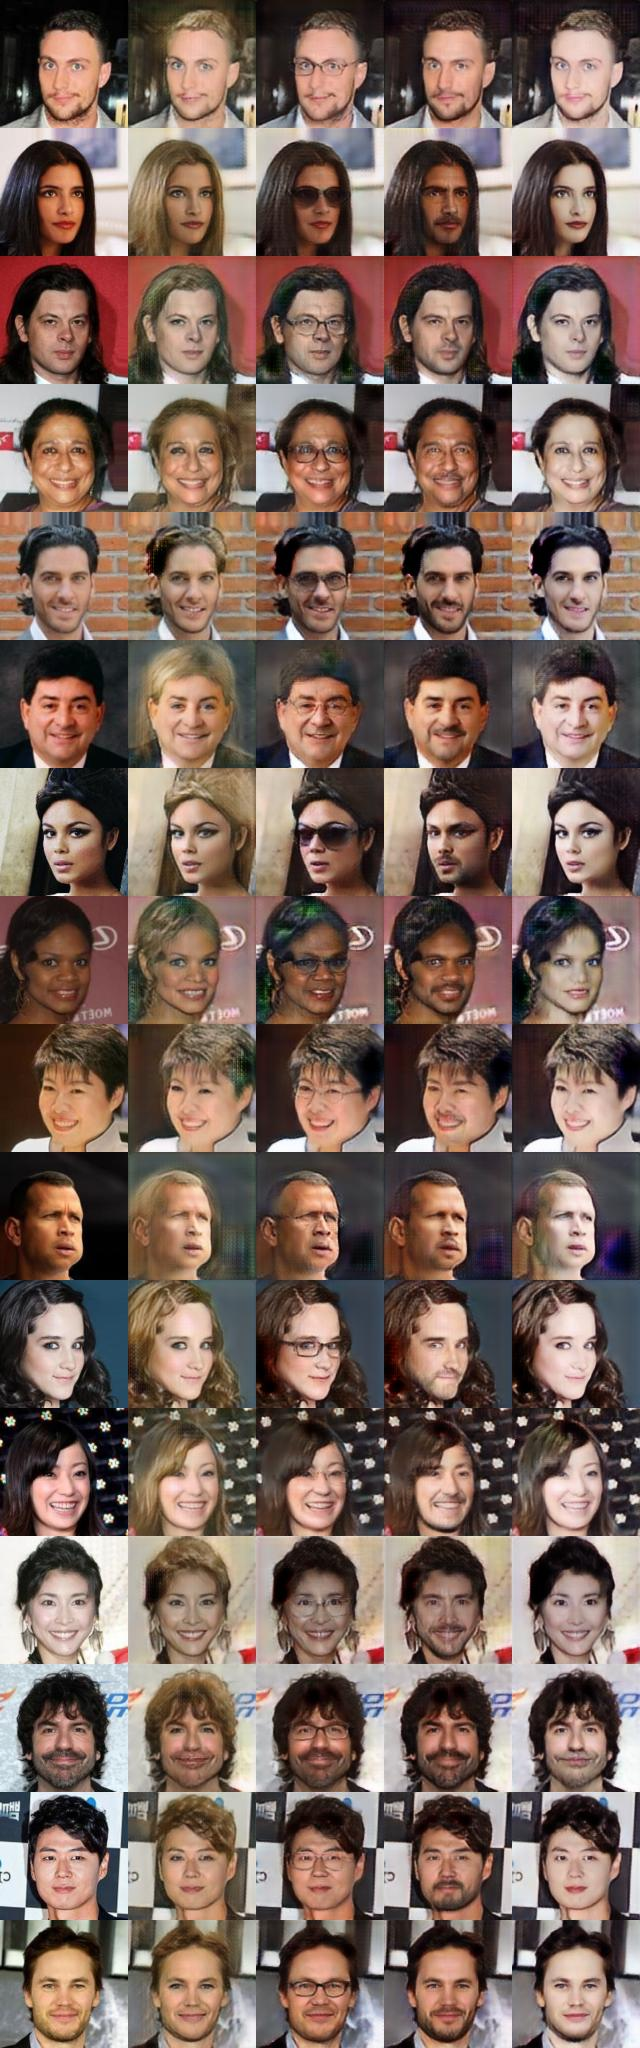
\includegraphics[width=0.49\linewidth,trim={0 59cm 0 0},clip]{figs/mwgan/baseline_050000-images.jpg}
%     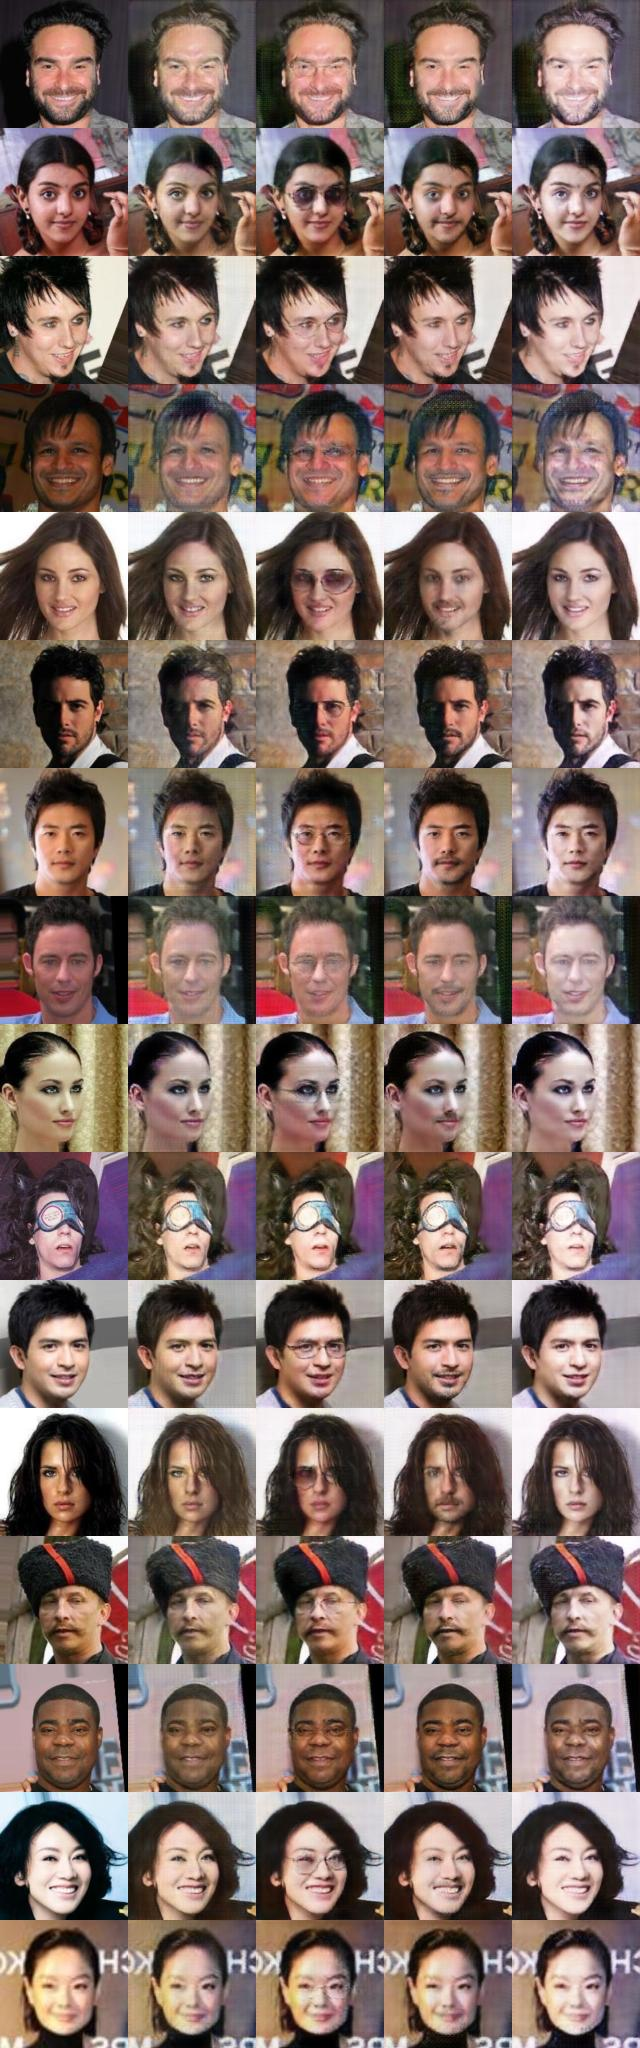
\includegraphics[width=0.49\linewidth,trim={0 58.7cm 0 0},clip]{figs/mwgan/046500-images.jpg}
%     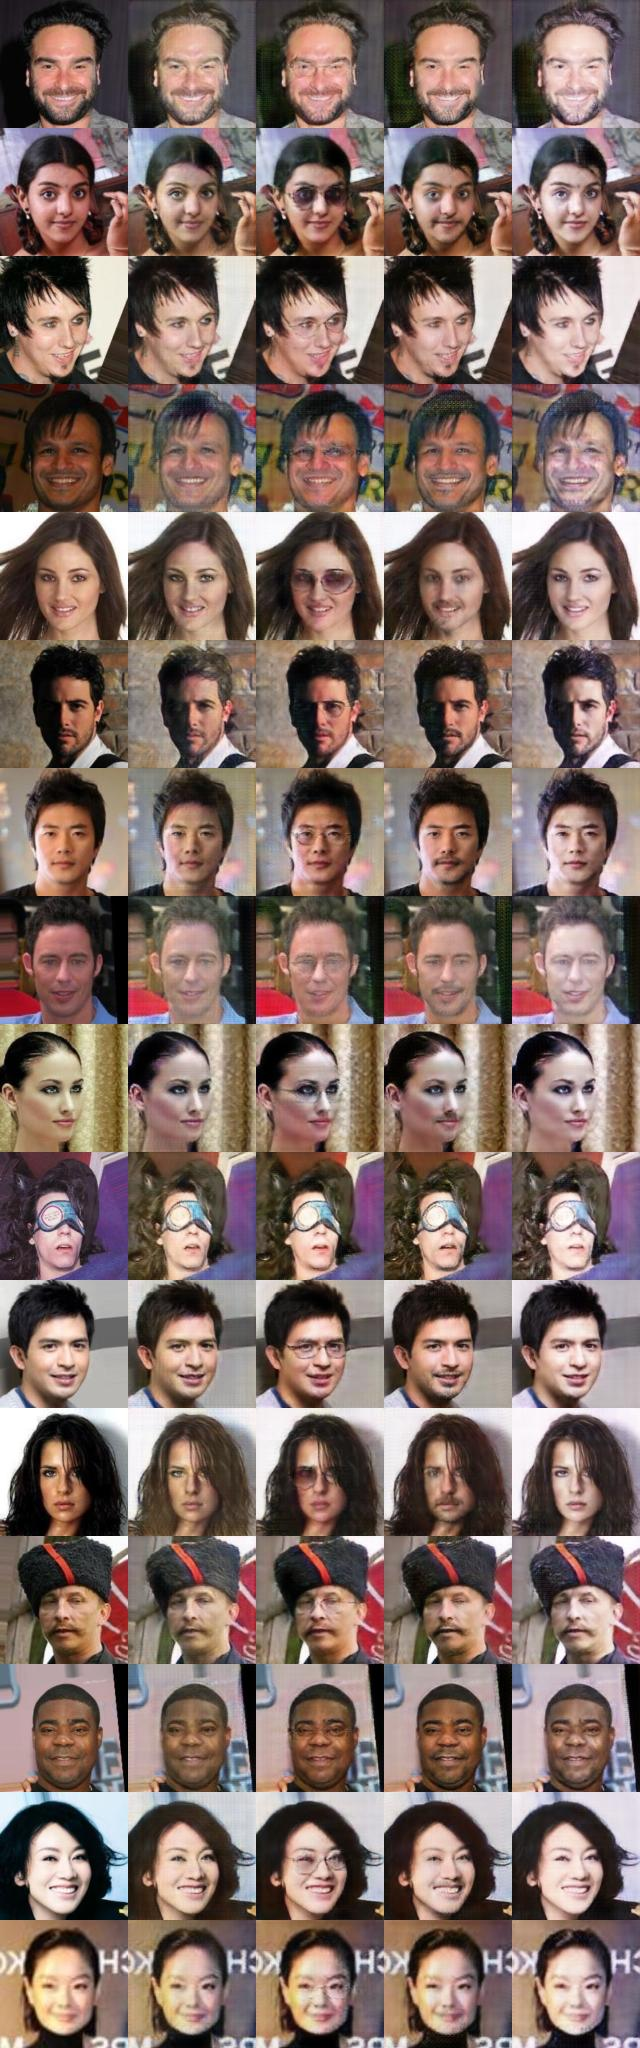
\includegraphics[width=0.49\linewidth,trim={0 0 0 58.7cm},clip]{figs/mwgan/046500-images.jpg}
%     % 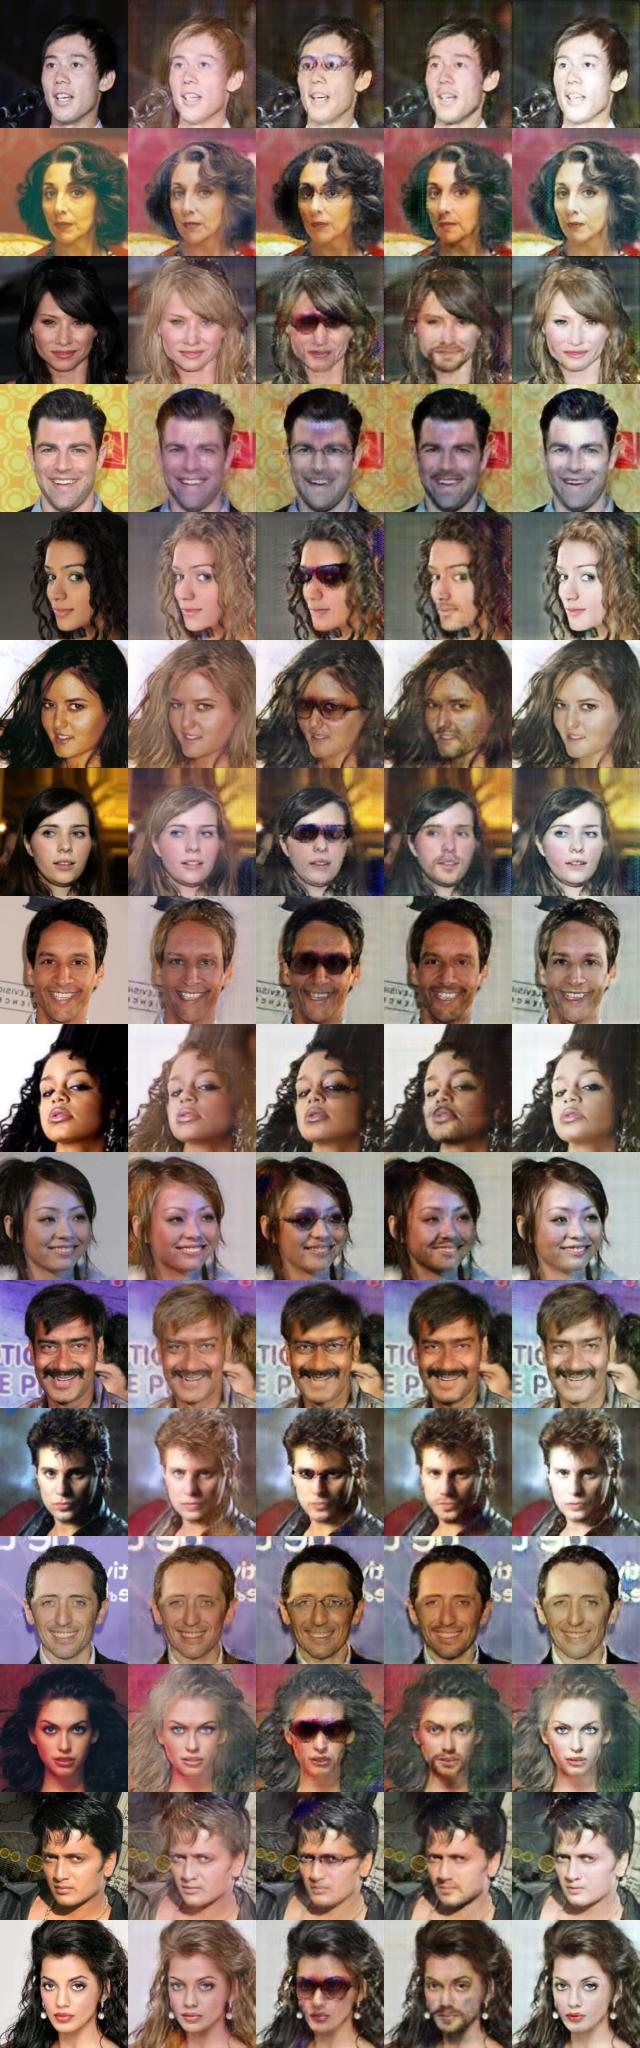
\includegraphics[width=0.49\linewidth,trim={0 63.5cm 0 0},clip]{figs/mwgan/demd_050000-images.jpg}
%     % 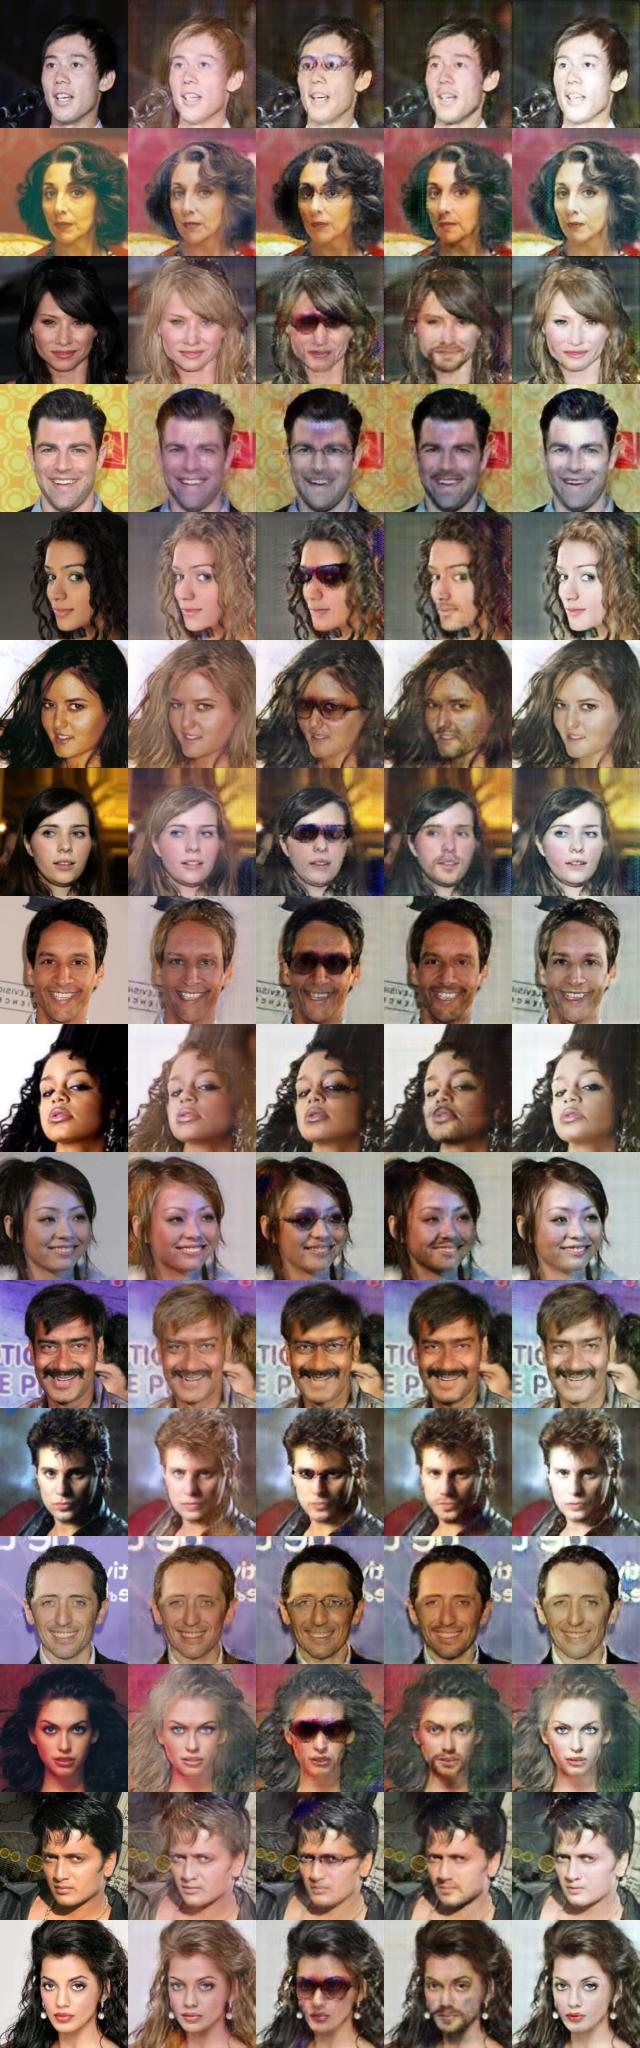
\includegraphics[width=0.49\linewidth,trim={0 63.5cm 0 0},clip]{figs/mwgan/demd_050000-images.jpg}
%     \caption{\footnotesize Six MWGAN+DEMD CelebA image translation results. Each row corresponds to a random sample in the validation set. The leftmost image is the original source image, and sequential columns represent translations to (1) Blonde Hair, (2) Glasses, (3) Mustache, and (4) Pale Skin.\ronak{put labels on top of images? add bar separating original and targets?}}
%     \label{fig:mwgan}
% \end{figure}

\begin{figure*}[t]
    \centering
    \scriptsize
    	Original \quad\; Blond Hair \quad\; Glasses \quad\; Moustache \quad\; Pale Skin \quad\quad Original \quad\; Blond Hair \quad\; Glasses \quad\; Moustache \quad\; Pale Skin \\
    	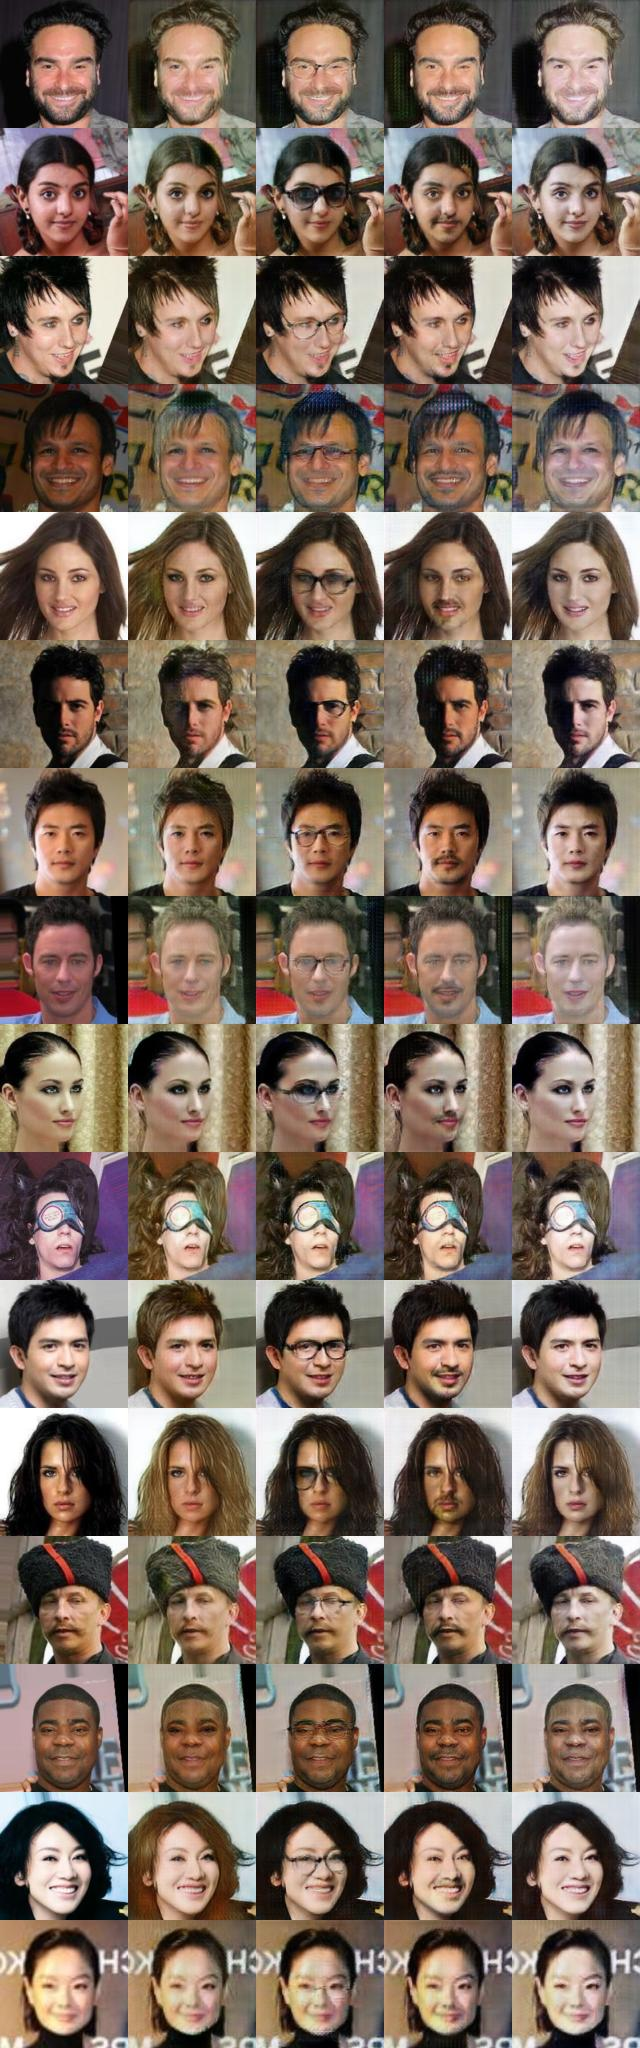
\includegraphics[width=0.49\linewidth,trim={0 58.7cm 0 0},clip]{6_demd/figs/mwgan/069500-images.jpg} 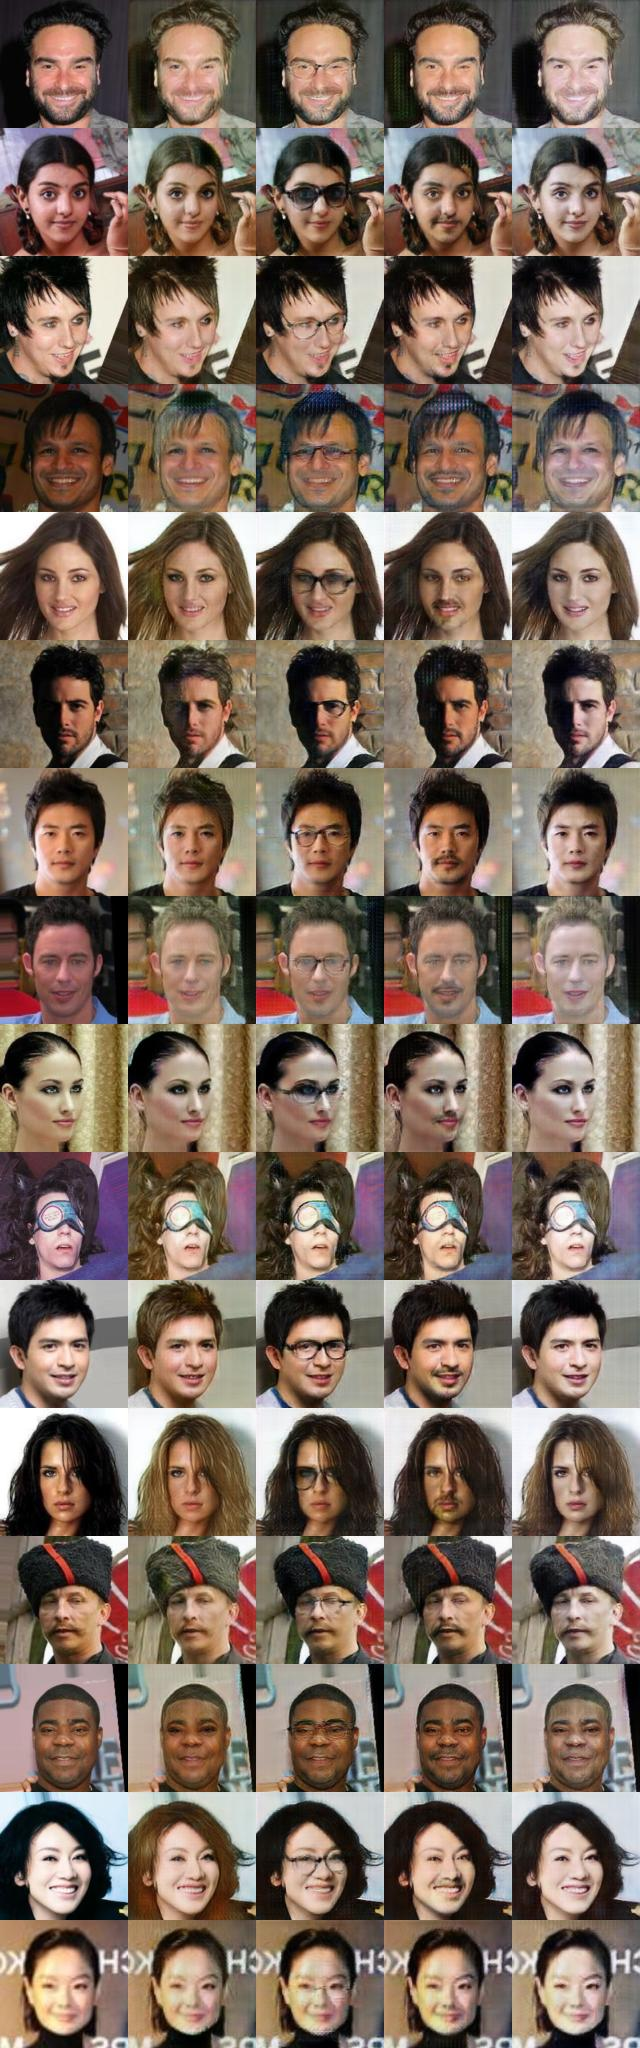
\includegraphics[width=0.49\linewidth,trim={0 0 0 58.7cm},clip]{6_demd/figs/mwgan/069500-images.jpg}
    \caption[Image translation on CelebA via d-MMOT]{Six MWGAN+DEMD CelebA image translation results. Each row corresponds to a random sample in the validation set. The leftmost image is the original source image, and sequential columns represent translations to (1) Blonde Hair, (2) Glasses, (3) Moustache, and (4) Pale Skin. Using DEMD as a relaxation to the Multiple Marginal Matching problem facilitates high quality images translation. For more results see Appendix~\ref{sec:app-mwgan}. }
    \label{fig:mwgan}
\end{figure*}


%%%%%%%%%%%%%%%%%%%%%%% OLD stuff
%%%%%%%%%%%%%%%%%%%%%%% OLD stuff
%%%%%%%%%%%%%%%%%%%%%%% OLD stuff
%%%%%%%%%%%%%%%%%%%%%%% OLD stuff



% \begin{table*}[!t] 
% 	\scriptsize
% 	\setlength\tabcolsep{4pt} % make LaTeX figure out width of inter-column spaces
% 	\caption{\footnotesize Fairness validation results, higher accuracy is better, Lower Fairness measures are better. Higher accuracies \textbf{(ACC)} with lower measures of max Demographic Parity Gap \textbf{(|DP|)},  Equalized Odds Gap \textbf{(|EO|)}, and \textbf{(DEMD)}. \vishnu{Other methods minimize DEMD better than DEMD algorithm itself? Kinda mixed message} \vishnu{Accuracy values should not be in bold. Infact, separate color needs to be used for accuracy column. The idea is that upto 2-4\% drop in accuracy is permissible as long as the fairness measures improve.} \vishnu{Accuracy values are different from this table to the next one! accuracy is kinda redundant information. Best if avoided or moved to the supplement}}
% 	\begin{tabular*}{\linewidth}{l *{3}{c}|*{3}{c}|*{3}{c}|*{3}{c}}
% 		\midrule%\midrule
% 		& \multicolumn{3}{c}{German} & \multicolumn{3}{c}{Adult} & \multicolumn{3}{c}{Crime}& \multicolumn{3}{c}{ACS-Employ} \\
% 		\cmidrule{2-4} \cmidrule{5-7} \cmidrule{8-10} \cmidrule{11-13}
% 		& ACC & |DP| & |EO| & DEMD & ACC  & |DP| & |EO| & DEMD & ACC & |DP| & |EO| & DEMD & ACC & |DP| & |EO| & DEMD \\ 
% 		\midrule
% 		None & 0.180 & 0.134 & 1.694 & 0.382 & 0.446 & 2.858 & 0.351 & 0.306 & 3.556 & 0.365 & 0.251 & 4.778 \\
% DP-Reg. & 0.169 & 0.128 & 1.600 & 0.383 & 0.446 & 2.832 & 0.362 & 0.250 & 3.705 & 0.477 & 0.276 & 5.024 \\
% EO-Reg. & 0.143 & 0.116 & 1.425 & 0.377 & 0.442 & 2.830 & 0.363 & 0.311 & 3.055 & 0.377 & 0.256 & 4.818 \\
% Bary & 0.177 & 0.134 & 1.645 & 0.362 & 0.442 & 2.811 & 0.377 & 0.256 & 2.726 & 0.571 & 0.497 & 4.376 \\
% DEMD & 0.145 & 0.117 & 1.443 & 0.364 & 0.438 & 2.688 & 0.288 & 0.361 & 3.101 & 0.334 & 0.236 & 3.598 \\
% % 		None & 0.77 & 0.17 & 0.11 & 1.69 & \textbf{0.84} & 0.18 & 0.13 & 1.69 & \textbf{0.84} & 0.38 & 0.45 & 2.86 & \textbf{0.80} & 0.35 & 0.31 & 3.56 \\
% % DP-Reg. & 0.77 & 0.16 & 0.10 & 1.50 & \textbf{0.84} & 0.17 & 0.13 & 1.60 & 0.83 & 0.37 & 0.44 & 2.65 & 0.79 & 0.36 & \textbf{0.25} & 3.71 \\
% % EO-Reg. & 0.75 & 0.20 & 0.11 & 1.59 & \textbf{0.84} & 0.14 & \textbf{0.12} & 1.43 & 0.83 & \textbf{0.35} & \textbf{0.43} & 2.54 & 0.79 & 0.53 & 0.36 & 3.06 \\
% % Bary & \textbf{0.79} & 0.27 & 0.17 & 1.50 & 0.81 & \textbf{0.13} & 0.14 & \textbf{0.99} & 0.81 & \textbf{0.35} & 0.44 & \textbf{2.61} & 0.79 & 0.38 & 0.26 & \textbf{2.73} \\
% % DEMD & 0.77 & \textbf{0.14} & \textbf{0.09} & \textbf{1.41} & \textbf{0.84} & 0.15 & \textbf{0.12} & 1.44 & 0.83 & 0.36 & 0.44 & 2.69 & \textbf{0.80} & \textbf{0.29} & 0.36 & 3.10 \\
% % 		None & XXYY & XXYY & XXYY & XXYY  & XXYY & XXYY & XXYY & XXYY & XXYY & XXYY & XXYY & XXYY & XXYY & XXYY & XXYY & XXYY \\
% % 		DP & XXYY & XXYY & XXYY & XXYY & XXYY & XXYY & XXYY & XXYY & XXYY & XXYY & XXYY & XXYY & XXYY & XXYY & XXYY & XXYY \\
% % 		EO & XXYY & XXYY & XXYY & XXYY & XXYY & XXYY & XXYY & XXYY & XXYY & XXYY & XXYY & XXYY & XXYY & XXYY & XXYY & XXYY \\
% % 		Bary & XXYY & XXYY & XXYY & XXYY & XXYY & XXYY & XXYY & XXYY & XXYY & XXYY & XXYY & XXYY & XXYY & XXYY & XXYY & XXYY \\
% % 		DEMD & XXYY & XXYY & XXYY & XXYY & XXYY & XXYY & XXYY & XXYY & XXYY & XXYY & XXYY & XXYY & XXYY & XXYY & XXYY & XXYY \\
% 		\midrule%\midrule
% 	\end{tabular*}
% 	\label{tab:fair_results}
% \end{table*} 

% \begin{table}[]
%     \centering
%     \begin{tabular}{c|cccc}
%         \toprule
%         $\lambda_{reg}$ & Acc & DP Gap & EO Gap & EMD \\
%         \midrule
%         0.00 & 0.776 & 0.665 & 0.723 & 3.352 \\
%         0.01 & 0.776 & 0.670 & 0.726 & 3.050 \\
%         0.02 & 0.776 & 0.474 & 0.527 & 2.317 \\
%         0.03 & 0.773 & 0.485 & 0.531 & 1.965 \\
%         0.04 & 0.763 & 0.506 & 0.540 & 1.575 \\
%         0.05 & 0.738 & 0.339 & 0.356 & 1.149 \\
%         0.06 & 0.670 & 0.178 & 0.200 & 0.662 \\
%         0.07 & 0.594 & 0.006 & 0.005 & 0.372 \\
%         0.08 & 0.590 & 0.000 & 0.000 & 0.031 \\
%         0.09 & 0.590 & 0.000 & 0.000 & 0.000 \\
%         0.10 & 0.590 & 0.000 & 0.000 & 0.000 \\\bottomrule
%     \end{tabular}
%     \caption{Outcome measures as a function of regularization parameter when our EMD regularizer is used.}
%     \label{tab:reg_sweep}
% \end{table}

% \begin{figure}
%     \centering
%     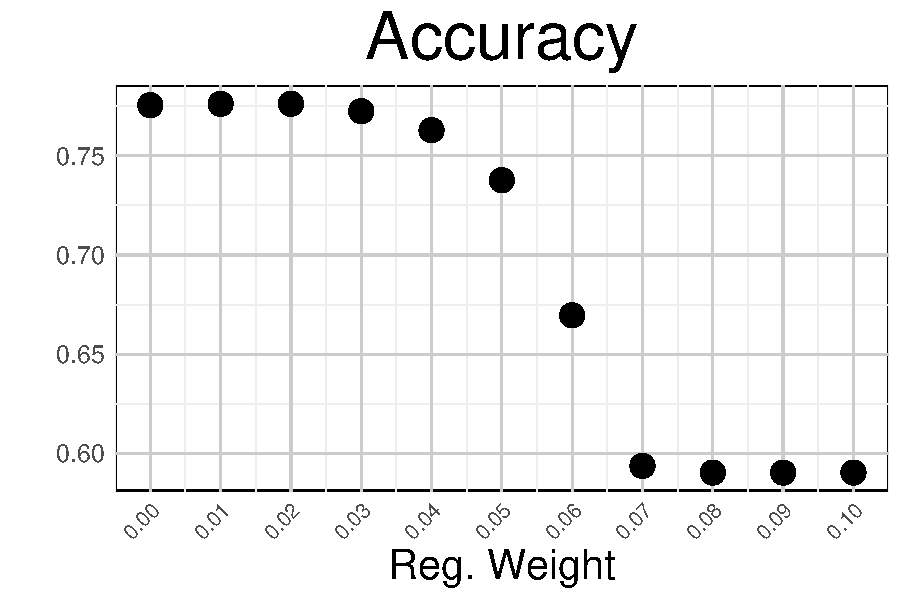
\includegraphics[width=0.24\columnwidth]{figs/regweights/lambdas_Acc.pdf}
%     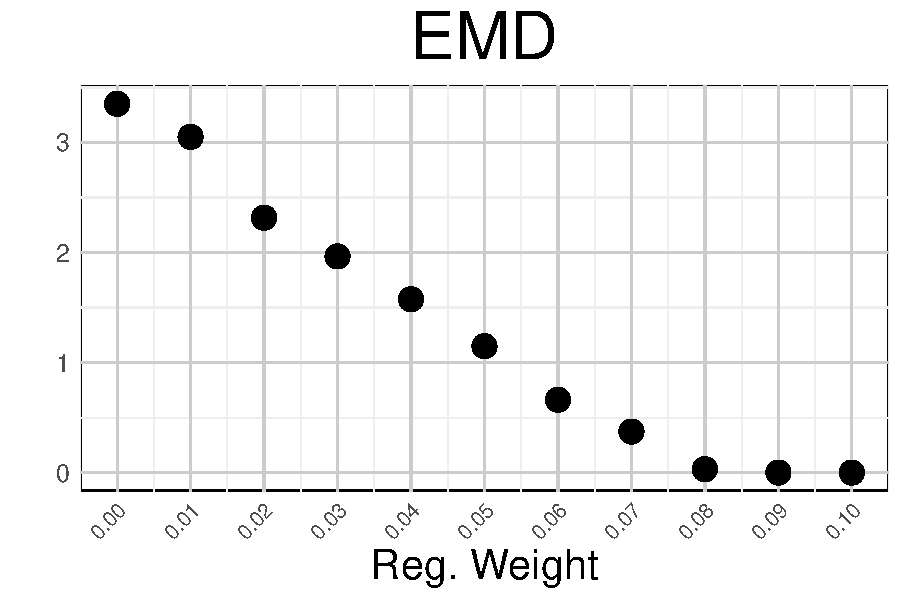
\includegraphics[width=0.24\columnwidth]{figs/regweights/lambdas_DEMD.pdf}
%     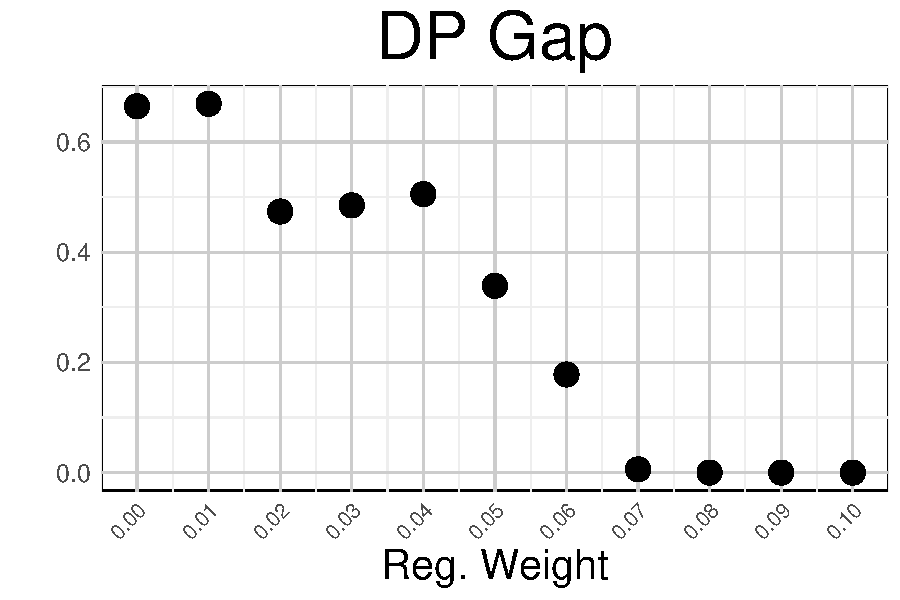
\includegraphics[width=0.24\columnwidth]{figs/regweights/lambdas_DPgap.pdf}
%     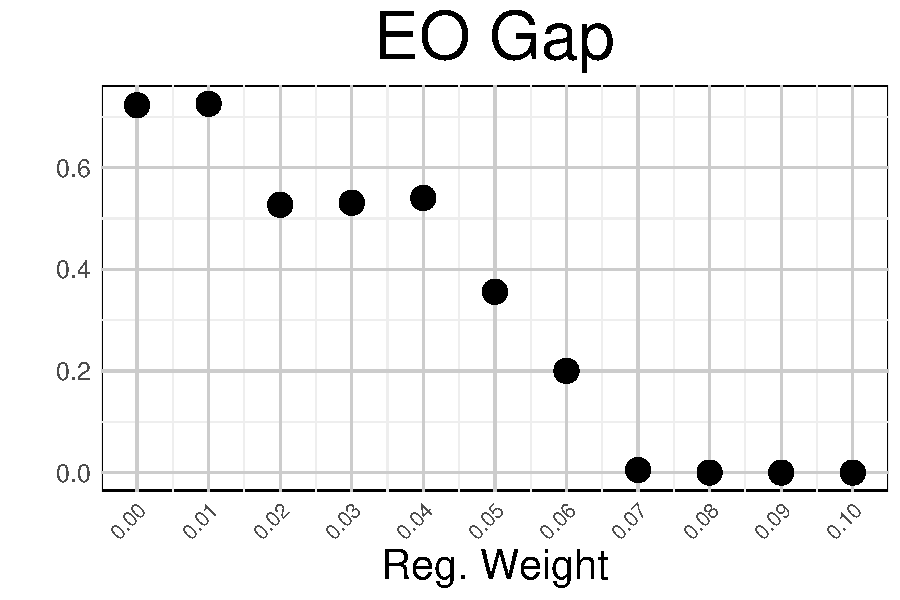
\includegraphics[width=0.24\columnwidth]{figs/regweights/lambdas_EOgap.pdf}
%     \caption{Outcome measures as a function of regularization parameter when our EMD regularizer is used. Output measures of fairness track the upstream EMD constraint, and follow the same accuracy-fairness tradeoff.}
%     \label{fig:reg_sweep}
% \end{figure}

% \begin{table*}[ht]
%     \centering\small
%     \begin{tabular}{llcccccc}
%     \toprule
%         RegType & $\lambda_{reg}$ & Total Acc & MinAcc & MaxAcc & $|DP_{max} - DP_{min}|$ & $|EO_{max} - EO_{min}|$ & D-EMD \\
%         \midrule
%         Log. Reg. & 0.0   & 0.786 & 0.699 & 0.867 & 0.474 & 0.522 & 3.331 \\
%                   & 0.001 & 0.786 & 0.708 & 0.878 & 0.481 & 0.526 & 3.332 \\
%                   & 0.01  & 0.590 & 0.200 & 0.878 & 0.000 & 0.000 & 0.044 \vspace{0.1in}\\
                  
%         2NN       & 0.0   & 0.795 & 0.600 & 0.856 & 0.371 & 0.327 & 3.265 \\
%                   & 0.001 & 0.794 & 0.600 & 0.878 & 0.354 & 0.335 & 2.976 \\
%                   & 0.01  & 0.648 & 0.200 & 0.878 & 0.108 & 0.100 & 0.062 \\
% \bottomrule\\
%     \end{tabular}
%     \caption{Validation results for various models and regularization weights on the ACS Income prediction task including demographic parity
% (DP) and equality of opportunity (EO) spreads. }
%     \label{tab:acsinc}
% \end{table*}


% \begin{table*}[ht]
%     \centering\small
%     \begin{tabular}{llcccccc}
%     \toprule
%         Model & $\lambda_{reg}$ & Total Acc & MinAcc & MaxAcc & $|DP_{max} - DP_{min}|$ & $|EO_{max} - EO_{min}|$ & D-EMD \\
%         \midrule
%         Log. Reg. & 0.0   & 0.786 & 0.699 & 0.867 & 0.474 & 0.522 & 3.331 \\
%                   & 0.001 & 0.786 & 0.708 & 0.878 & 0.481 & 0.526 & 3.332 \\
%                   & 0.01  & 0.590 & 0.200 & 0.878 & 0.000 & 0.000 & 0.044 \vspace{0.1in}\\
                  
%         2NN       & 0.0   & 0.795 & 0.600 & 0.856 & 0.371 & 0.327 & 3.265 \\
%                   & 0.001 & 0.794 & 0.600 & 0.878 & 0.354 & 0.335 & 2.976 \\
%                   & 0.01  & 0.648 & 0.200 & 0.878 & 0.108 & 0.100 & 0.062 \\
% \bottomrule\\
%     \end{tabular}
%     \caption{Validation results for various models and regularization weights on the ACS Income prediction task including demographic parity
% (DP) and equality of opportunity (EO) spreads. }
%     \label{tab:acsinc}
% \end{table*}

% \begin{table*}[ht]
%     \centering\small
%     \begin{tabular}{llcccccc}
%     \toprule
%         Model & $\lambda_{reg}$ & Total Acc & MinAcc & MaxAcc & $|DP_{max} - DP_{min}|$ & $|EO_{max} - EO_{min}|$ & D-EMD \\
%         \midrule
%         Log. Reg.  & 0.0  & 0.769 & 0.500 & 0.824 & 0.194 & 0.194 & 2.200  \\
%                   & 0.01 & 0.769 & 0.500 & 0.824 & 0.194 & 0.185 & 2.124  \\
%                   & 0.1  & 0.546 & 0.500 & 0.632 & 0.000 & 0.000 & 0.093  \vspace{0.1in}\\
%         2NN        & 0.0 & 0.806 & 0.744 & 1.000 & 0.167 & 0.176 & 2.844  \\
%                   & 0.01 & 0.806 & 0.774 & 1.000 & 0.165 & 0.180 & 2.644  \\
%                   & 0.1 & 0.645 & 0.500 & 0.708 & 0.244 & 0.203 & 0.059  \\
% \bottomrule\\
%     \end{tabular}
%     \caption{Validation results for various models and regularization weights on the ACS Employment prediction task including demographic parity
% (DP) and equality of opportunity (EO) spreads.}
%     \label{tab:acsemp}
% \end{table*}